\documentclass[xodstep]{wnspt}

\author   {Tetiana Mossur}
\nralbumu {76716}
\kierunek {Informatyka}
\specjalnosc {Programowanie}
\date     {2024}
\miejsce {Cz\k{e}stochowa}
%\instytut {Zak\l{}adzie Informatyki Stosowanej}
\opiekun  {dr hab. Andrzeja Zbrzeznego}

\usepackage{amsmath}
\usepackage{amsfonts}
\usepackage{amsthm}
\usepackage{amssymb}
\usepackage[T1]{fontenc}
\usepackage[utf8]{inputenc}
\usepackage[polish]{babel}
\usepackage{polski}
\usepackage{csquotes}
\usepackage{times}
\usepackage{colortbl}
\usepackage{graphicx}
\usepackage{url}
\usepackage{setspace}
\usepackage{indentfirst}
\usepackage{listingsutf8}
\usepackage{beramono}
\usepackage[%
backend=biber,refsegment=section,
defernumbers=true,
]{biblatex}

\usepackage{fontspec}
\setmainfont{Carlito}

\usepackage{macros}

\defbibfilter{articles_and_proceedings}{
	type=article or
	type=inproceedings
}

\bibliography{literatura}

\lstset{ %
language=Python,                  % choose the language of the code
basicstyle=\ttfamily,           % the fonts that are used for the code
numbers=left,                   % where to put the line-numbers
numberstyle=\footnotesize,      % the size of the fonts that are used for the line-numbers
stepnumber=1,                   % the step between two line-numbers. If it's 1 each line will be
numbersep=5pt,                  % how far the line-numbers are from the code
showspaces=false,               % show spaces adding particular underscores
showstringspaces=false,         % underline spaces within strings
showtabs=false,                 % show tabs within strings adding particular underscores
frame=single,                   % adds a frame around the code
tabsize=4,                      % sets default tabsize to 2 spaces
captionpos=b,                   % sets the caption-position to bottom
breaklines=true,                % sets automatic line breaking
breakatwhitespace=false,        % sets if automatic breaks should only happen at whitespace
escapeinside={\%*}{*)}          % if you want to add a comment within your code
}

\newcommand{\R}{mathbb{R}}

\renewcommand{\lstlistlistingname}{Spis listingów}
\renewcommand{\lstlistingname}{Listing}

\newtheorem{lemat}{Lemat}
\newtheorem{twierdzenie}{Twierdzenie}

\title{Efektywność SMT solverów dla klasycznych problemów NP-trudnych
\\{~}
\\{~}
Effectiveness of SMT solvers for classical NP-hard problems}

\frenchspacing

\begin{document}
\begin{abstract}
Celem niniejszej pracy jest analiza i ocena efektywności SMT solverów w rozwiązywaniu klasycznych problemów zaliczanych do klasy NP-trudnych. Przełom w informatyce teoretycznej sprawił, że tego rodzaju zagadnienia stały się przedmiotem intensywnych badań. Niniejsza praca skupi się na zrozumieniu, jak SMT (Satisfiability Modulo Theories) solvery, będące potężnym narzędziem w dziedzinie rozstrzygania logicznego, radzą sobie z tymi wyjątkowo wymagającymi problemami.
Przedmiotem badań będą klasyczne problemy NP-trudne, a celem jest zbadanie i porównanie wydajności trzech SMT solverów - Z3, Yices i CVC5 - w kontekście rozwiązywania konkretnych problemów. Wybór tych narzędzi wynika z ich popularności, wszechstronności i aktywnego udziału w społeczności badawczej.

\end{abstract}

\keywords{SMT, SMT-solvery, Z3, Yices, CVC5, Python, złożoność obliczeniowa, NP-hard}

\maketitle
\onehalfspacing
%\setlength{\footskip}{20pt}

\introduction
W niektórych dziedzinach informatyki, takich jak formalna weryfikacja sprzętu i oprogramowania, wiele istotnych problemów można zredukować do sprawdzenia spełnialności formuły w pewnej logice. Kilka z tych problemów można naturalnie sformułować jako problemy spełnialności w logice propozycjonalnej i rozwiązać bardzo efektywnie przy użyciu nowoczesnych solverów SAT. Inne problemy są bardziej zwięźle sformułowane w logikach klasycznych, takich jak logika pierwszego lub wyższego rzędu, o bardziej złożonym języku, który obejmuje zmienne niebędące wartościami logicznymi, funkcje i symbole predykatów oraz kwantyfikatory. Oczywiście istnieje kompromis między złożonością logiki a zdolnością do automatycznego sprawdzania spełnialności jej formuł.

Praktyczny kompromis można osiągnąć za pomocą fragmentów logiki pierwszego rzędu, które są ograniczone syntaktycznie, na przykład przez zezwolenie tylko na pewne klasy formuł, lub semantycznie, poprzez ograniczenie interpretacji niektórych funkcji i symboli predykatów, lub obie te opcje jednocześnie. Takie ograniczenia mogą uczynić problem spełnialności rozstrzygalnym i, co ważniejsze, umożliwić rozwijanie specjalistycznych procedur spełnialności, które wykorzystują właściwości fragmentu logiki z dużą korzyścią dla wydajności praktycznej, nawet w przypadku wysokiej złożoności obliczeniowej dla najgorszych scenariuszy (worst-case computational complexity). Kiedy są zaangażowane ograniczenia semantyczne, mogą one być pojęte jako ograniczenie interpretacji do modeli pewnej teorii tła (background theory) (np. teorii równości, liczb całkowitych, liczb rzeczywistych, tablic, list itp.). W takich przypadkach mówimy o Spełnialności Moduło Teorii (SMT).

W oparciu o klasyczne rozwiązania dotyczące procedur decyzyjnych dla rozumowania pierwszego rzędu, a także ogromny rozwój technologii rozwiązywania SAT w ciągu minionych dwóch dekad,
SMT rozwinęło się przez ostatnie lata w bardzo aktywny obszar badawczy, którego cechą charakterystyczną jest wykorzystywanie metod wnioskowania, właściwych logicznym teoriom o dużym znaczeniu dla problemów stosowanych.
Dzięki postępowi w badaniach i technologii SMT, istnieje obecnie kilka potężnych i zaawansowanych solverów SMT (np. Alt-Ergo, Beaver, Boolector, CVC5, MathSAT5, openSMT, SMTInterpol, SONOLAR, STP, veriT, Yices i Z3), które są wykorzystywane w szybko rosnącym szeregu aplikacji. Wśród nich znajdują się obecnie m.in. weryfikacja procesorów, badanie równoważności, ograniczone i nieograniczone sprawdzanie modeli, abstrakcja predykatów, analiza statyczna, automatyczne generowanie przypadków testowych, sprawdzanie typów, harmonogramowanie i optymalizacja.
Ostatnie osiągnięcia w dziedzinie SMT były spowodowane kilkoma czynnikami, w tym skupieniem się na podstawowych teoriach i klasach problemów występujących w praktyce, dostosowanie technologii SAT do potrzeb SMT oraz innowacje w zakresie algorytmów i struktur danych \cite{Clarke18}.

Celem niniejszej pracy jest zbadanie skuteczności SMT solverów w rozwiązywaniu dwunastu klasycznych problemów NP-trudnych, a mianowicie: Ścieżka Hamiltona, Izomorfizm grafów, Pokrycie wierzchołkowe (ang. Vertex Cover), Problem kliki (ang. The maximum clique size problem), Problem pokrycia zbioru (ang. Set Cover), Problem maksymalnego zbioru niezależnego (ang. Maximum Independent Set), Problem Komiwojażera, Kolorowanie grafu, Problem sumy podzbioru (ang. SubsetSum), Drzewo Steinera (ang. Steiner Tree), Problem plecakowy, Problem najbliższego ciągu (ang. Closest string).

W pierwszym rozdziale zawarłam teoretyczne fundamenty Satisfiability Modulo Theories (SMT), wprowadzając czytelnika w główne aspekty tej dziedziny. Omówiłam kluczowe pojęcia, biorąc pod uwagę rozwój SMT-solverów i ich praktyczne zastosowania w realnych sytuacjach, takich jak te związane z klasą problemów NP-trudnych. 

Drugi rozdział przedstawia podstawowe pojęcia złożoności obliczeniowej oraz koncepcji spełnialności, dwóch kluczowych aspektów niezbędnych do zrozumienia, czym są problemy obliczeniowe w kontekście SMT. Następnie dokonywana jest definicja klasy problemów NP-trudnych, które stanowią centralny temat niniejszej pracy magisterskiej.

W rozdziale trzecim zawarłam szczegółowy przegląd trzech popularnych SMT-solverów: Z3, Yices i CVC5, podkreślając ich cechy, mocne strony i potencjalne ograniczenia. Czytelnik zdobywa wgląd w różnice między tymi narzędziami, co stanowi podstawę dla późniejszych badań.

Rozdział czwarty skupia się na przedstawieniu 12 klasycznych problemów NP-trudnych, a następnie opisuje sposób ich kodowania w języku Python.

Rozdział piąty poświęcony jest praktycznym eksperymentom, wykorzystując wyżej przedstawione solvery do rozwiązania wybranych problemów obliczeniowych. Analiza wyników pozwoli określić efektywność każdego z nich i wyciągnąc wnioski co do ich zastosowania.

\chapter{Teoretyczne podstawy SMT i klasy NP-hard}
\section{Wymagania biznesowe}
\section{Słownik skrótów i pojęć}
\cite{java_fundamentals}
\section{Wymagania funkcjonalne użytkowników}
%\subsection*{Hierarchia grup użytkowników przedstawiona graficznie}
\subsection{Wymagania funkcjonalne użytkownika niezarejestrowanego}
\subsection{Wymagania funkcjonalne użytkownika zarejestrowanego}
\subsection{Wymagania funkcjonalne administratora}
\subsection{Wymagania funkcjonalne dziennikarz}
\subsection{Wymagania funkcjonalne marketing}
\subsection{Wymagania funkcjonalne specjalista danych}
\subsection{Wymagania funkcjonalne super administratora}
\section{Wymagania niefunkcjonalne użytkowników}
\section{Wymagania niefunkcjonalne systemowe}
\section{Reguły biznesowe}
\cite{java17doc}


\chapter{Problemy NP-trudne}

Załóżmy, że jesteśmy menedżerem logistyki, który musi zoptymalizować harmonogram dostaw towarów przez park pojazdów w warunkach ograniczonej sieci dystrybucyjnej obejmującej całe miasto. To pozornie rutynowe zadanie, po bliższym przyjrzeniu się, okazuje się być złożonym problemem optymalizacji kombinatorycznej, charakteryzującym się potrzebą minimalizacji kosztów paliwa, skrócenia czasu podróży i maksymalizacji przepustowości dostaw.

W poszukiwaniu optymalnego rozwiązania mamy do czynienia ze stale rosnącym zestawem zmiennych, w tym nieprzewidywalną dynamiką ruchu, różnymi rozmiarami paczek i dynamicznymi zmianami popytu ze strony klientów. Każda decyzja o ustaleniu konkretnych tras dostawy lub nadaniu priorytetu określonym miejscom docelowym powoduje eksplozję kombinatorycznych możliwości, zmieniając problem optymalizacji logistycznej w przykład problemu NP-trudnego.

Z perspektywy obliczeniowej, problemy NP-trudne są klasą problemów, dla których nie istnieje algorytm wielomianowy, który może zapewnić optymalne rozwiązanie we wszystkich przypadkach. Złożoność ta jest wyraźnie widoczna w problemach takich jak optymalizacja tras, gdzie ogromna przestrzeń rozwiązań nie pozwala na proste rozwiązanie. Złożoność takich problemów logistycznych odzwierciedla szersze trudności występujące w problemach NP-trudnych w różnych obszarach obliczeniowych i optymalizacyjnych.

\section{Złożoność obliczeniowa}

\section{Problem spełnialnośći}

\section{Definicja klasy problemów NP-trudnych}



%\begin{lstlisting}
%\end{lstlisting}
 

\chapter{Opis wykorzystywanych narzędzi}
%Rozdział opisuje zastosowanie 

\section{Z3 Solver}
Z3 to wydajny SMT solver dostępny bezpłatnie przez Microsoft Research. Z3 jest solverem dla logiki symbolicznej, będącej podstawą wielu narzędzi inżynierii oprogramowania. Solwery SMT polegają na ścisłej integracji wyspecjalizowanych silników walidacyjnych. Każdy silnik jest elementem ogólnej struktury i implementuje wyspecjalizowane algorytmy. Przykładowo, silnik Z3 dla arytmetyki obejmuje Simplex, cięcia i rozumowanie wielomianowe, podczas gdy silnik dla obsługi ciągów znaków i wyrażeń regularnych korzysta z metod symbolicznych pochodnych języków regularnych. Wspólną cechą wielu algorytmów jest sposób, w jaki wykorzystują dwoistość między znajdowaniem rozwiązań spełniających a dowodów odrzucających. Solver ten integruje również silniki do wnioskowań globalnych i lokalnych oraz globalnej propagacji.
Z3 jest używany w szerokim zakresie zastosowań inżynierii oprogramowania, obejmując weryfikację programów, walidację kompilatorów, testowanie, fuzzing przy użyciu dynamicznego wykonywania symbolicznego, rozwój oprogramowania oparty na modelach, weryfikację sieci i optymalizację.
Z3 może być zbudowany przy użyciu Visual Studio, pliku Makefile lib CMake. Zapewnia obsługę wielu języków programowania, w tym .NET, C, C++, Java, OCaml, Web Assembly i Python.

\subsection{Architektura systemu}
	\begin{figure}
	\centering
	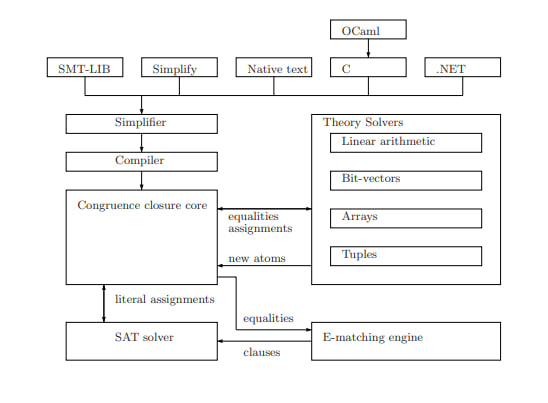
\includegraphics[width=0.7\linewidth]{screenshot001}
	\caption{}
	\label{fig:screenshot001}
	\end{figure}
\text{Z3 integruje nowoczesny solver SAT oparty na DPLL, bazowy solwer dla teorii, który obsługuje równości i funkcje nieinterpretowane, specjalistyczne silniki (dla arytmetyki, tablic itp.) oraz maszynę abstrakcyjną E-matching (dla kwantyfikatorów). Z3 jest zaimplementowany w C++. Schematyczny przegląd Z3 pokazano na poniższym rysunku.}

\textbf{Simplifier}. Formuły wejściowe są najpierw przetwarzane przy użyciu niekompletnego, ale wydajnego uproszczenia. Simplifier stosuje standardowe zasady redukcji algebraicznej, takie jak $p \land true \implies p$, ale także wykonuje ograniczone uproszczenie kontekstowe, identyfikując definicje równościowe w danym kontekście i redukuje pozostałą formułę przy użyciu definicji, na przykład $x = 4 \land q(x) \implies x = 4 \land q(4)$. Trywialnie spełnialny spójnik $x = 4$ nie jest kompilowany do jądra, ale zachowany poza nim na wypadek, gdyby klient wymagał modelu do obliczenia x.

\textbf{Compiler}. Uproszczona abstrakcyjna reprezentacja drzewa składniowego formuły jest przekształcana w inną strukturę danych, składającą się z zestawu klauzul i węzłów domknięcia kongruencji.


\section{Yices Solver}
sdcssdsdf

\section{CVC5 Solver}
sdsdcfsdfcdsf
\chapter{Kodowanie problemów}
\chapter{Eksperymenty i analiza wyników}

\section{Przeprowadzenie eksperymentów i zbieranie danych}

\section{Analiza zebranych danych i porównanie efektywności solverów}

\section{Identyfikacja czynników wpływających na efektywność}




\summary
Celem mojej pracy było zapoznanie czytelnika z ... 
Uważam, że udało mi się zrealizować ten cel. Starałem się opisać zarówno ...

% załączniki (opcjonalnie):
\appendix
\chapter{Tytuł załącznika jeden}
Treść załącznika jeden.

\chapter{Tytuł załącznika dwa}
Treść załącznika dwa.

%\bibliographystyle{plain}
%\bibliography{literatura}

\printbibliography[filter=articles_and_proceedings,title={Bibliografia - artykuły i referaty konferencyjne}]
\printbibliography[type=book,title={Bibliografia - książki}]
\printbibliography[type=misc,title={Bibliografia - strony internetowe}]

% spis tabel (jeżeli jest potrzebny):
\listoftables 

% spis rysunków (jeżeli jest potrzebny):
\listoffigures

% spis listingów (jeżeli jest potrzebny):
\lstlistoflistings

\end{document}
